% future/tm.tex

\section{Transactional Memory}
\label{sec:future:Transactional Memory}

데이터베이스 바깥의 영역에서 트랜잭션을 사용하자는 아이디어는 수십년 전으로
거슬러 오르는데~\cite{DBLomet1977SIGSOFT}, 이 아이디어는 데이터베이스에서와
데이터베이스 외에서의 트랜잭션에 대해 데이터베이스 외에서의 트랜잭션은
데이터베이스 트랜잭션을 정의하는 성질인 ``ACID'' 에서 ``D'' 를 빼냅니다.
하드웨어에서 메모리 기반의 트랜잭션, 또는 ``트랜잭셔널 메모리'' (TM) 을
지원하려는 아이디어는 최근의 것입니다만~\cite{Herlihy93a}, 안타깝게도 실제 많이
사용되는 하드웨어에서의 그런 트랜잭션의 지원은 그와 비슷한 것들에 대한 제안은
계속 있어왔지만~\cite{JMStone93}, 곧바로 이루어지지는 않았습니다.
그로부터 그렇게 오래지 않아, Shavit 과 Touitou 는 일반적으로 사용되는
하드웨어에서 동작할 수 있는, 메모리 접근 순서를 조정해서 소프트웨어만으로
이루어진 트랜잭셔널 메모리 구현 (STM) 을 제안했습니다.
이 제안은 여러 해동안 질질 끌려졌는데, 어쩌면 연구자 커뮤니티들의 관심은
non-blocking 동기화 (Section~\ref{sec:advsync:Non-Blocking Synchronization} 을
참고하세요) 에 열중되었기 때문일 수도 있습니다.
\iffalse

The idea of using transactions outside of databases goes back many
decades~\cite{DBLomet1977SIGSOFT}, with the key difference between
database and non-database transactions being that non-database transactions
drop the ``D'' in the ``ACID'' properties defining database transactions.
The idea of supporting memory-based transactions, or ``transactional memory''
(TM), in hardware
is more recent~\cite{Herlihy93a}, but unfortunately, support for such
transactions in commodity hardware was not immediately forthcoming,
despite other somewhat similar proposals being put forward~\cite{JMStone93}.
Not long after, Shavit and Touitou proposed a software-only implementation
of transactional memory (STM) that was capable of running on commodity
hardware, give or take memory-ordering issues.
This proposal languished for many years, perhaps due to the fact that
the research community's attention was absorbed by non-blocking
synchronization (see Section~\ref{sec:advsync:Non-Blocking Synchronization}).
\fi

하지만 세기가 변하면서, TM 은 일부 주의의 목소리를 받기
시작했고~\cite{Blundell2005DebunkTM,McKenney2007PLOSTM}, 2000년부터 2009년
사이의 중반 쯤에는 몇가지 경고의 목소리에도
불구하고~\cite{MauriceHerlihy2005-TM-manifesto.pldi,DanGrossman2007TMGCAnalogy},
그 관심의 수준이 ``열광적'' 이라 할 수 있게 되었습니다.
\iffalse

But by the turn of the century, TM started receiving
more attention~\cite{Martinez01a,Rajwar01a}, and by the middle of the
decade, the level of interest can only be termed
``incandescent''~\cite{MauriceHerlihy2005-TM-manifesto.pldi,
DanGrossman2007TMGCAnalogy}, despite a few voices of
caution~\cite{Blundell2005DebunkTM,McKenney2007PLOSTM}.
\fi

TM 에 대한 기본 아이디어는 한 섹션의 코드를 어토믹하게 수행해서 다른 쓰레드가
그 중간의 상태를 볼 수 없게 하자는 것입니다.
그렇게, TM 의 의미는 간단히 각각의 트랜잭션을 반복적으로 획득할 수 있는 글로벌
락의 획득과 해제로 감싸는 것으로, 성능과 확장성이 처참해지긴 하겠지만, 구현될
수 있습니다.
하드웨어에서든 소프트웨어에서든 TM 구현에서는 피할 수 없는 복잡성은 동시적인
트랜잭션들이 안전하게 병렬적으로 수행될 수 있는지에 대한 파악입니다.
이 파악은 동적으로 이루어지기 때문에, 충돌하는 트랜잭션들은 취소되거나
``롤백''될 수 있고, 일부 구현에서는, 이 실패한 모드가 프로그래머에게 보여질 수
있습니다.
\iffalse

The basic idea behind TM is to execute a section of
code atomically, so that other threads see no intermediate state.
As such, the semantics of TM could be implemented
by simply replacing each transaction with a recursively acquirable
global lock acquisition and release, albeit with abysmal performance
and scalability.
Much of the complexity inherent in TM implementations, whether hardware
or software, is efficiently detecting when concurrent transactions can safely
run in parallel.
Because this detection is done dynamically, conflicting transactions
can be aborted or ``rolled back'', and in some implementations, this
failure mode is visible to the programmer.
\fi

트랜잭션 롤백은 트랜잭션 크기가 줄어듦에 따라 발생률이 줄어들 것이기 때문에, TM
은 스택, 큐, 해시 테이블, 탐색 트리들과 같은 데에 사용되는 링크드 리스트 제어와
같이 작은 크기의 메모리 기반 오퍼레이션들에 매력적일 수 있습니다.
하지만, I/O 와 프로세스 생성과 같은 메모리 기반이 아닌 오퍼레이션들을 포함하는
것들과 같은, 커다란 트랜잭션들에 TM 을 적용하기는 어렵습니다.
다음 섹션들은 ``Transactional Memory
Everywhere''~\cite{PaulEMcKenney2009TMeverywhere} 의 커다란 비전을 위해
존재하는 현재의 극복해야할 사항들을 알아봅니다.
Section~\ref{sec:future:Outside World} 은 바깥의 것들과 상호동작하는 데에
나타나는 문제점들을 알아보고,
Section~\ref{sec:future:Process Modification} 는 프로세스 수정 기능들과의
상호동작을 보며,
Section~\ref{sec:future:Synchronization} 는 다른 동기화 기능들과의 상호
동작들을 살펴보며, 마지막으로
Section~\ref{sec:future:Discussion} 에서 일부 토의와 함께 마무리 합니다.
\iffalse

Because transaction roll-back is increasingly unlikely as transaction
size decreases, TM might become quite attractive for small memory-based
operations,
such as linked-list manipulations used for stacks, queues, hash tables,
and search trees.
However, it is currently much more difficult to make the case for large
transactions, particularly those containing non-memory operations such
as I/O and process creation.
The following sections look at current challenges to the grand vision of
``Transactional Memory Everywhere''~\cite{PaulEMcKenney2009TMeverywhere}.
Section~\ref{sec:future:Outside World} examines the challenges faced
interacting with the outside world,
Section~\ref{sec:future:Process Modification} looks at interactions
with process modification primitives,
Section~\ref{sec:future:Synchronization} explores interactions with
other synchronization primitives, and finally
Section~\ref{sec:future:Discussion} closes with some discussion.
\fi

\subsection{Outside World}
\label{sec:future:Outside World}

Donal Knuth 의 말을 인용하면:
\iffalse

In the words of Donald Knuth:
\fi

\begin{quote}
	많은 컴퓨터 사용자들이 입력과 출력은 ``진짜 프로그래밍'' 의 실제 부분은
	아니고, 그것들은 그저 기계로 정보를 넣고 그로부터 정보를 뽑아내기 위해
	(불행히도) 반드시 해야만 하는것들이라고 느낍니다.
	\iffalse

	Many computer users feel that input and output are not actually part
	of ``real programming,'' they are merely things that (unfortunately)
	must be done in order to get information in and out of the machine.
	\fi
\end{quote}

우리가 입력과 출력이 ``진짜 프로그래밍'' 이라 믿든 아니라 믿든, 대부분의 컴퓨터
시스템들에 있어서, 바깥 세상과의 상호작용이 첫번째 중요도의 요구사항임은
사실입니다.
따라서 이 섹션은 트랜잭셔널의, I/O 오퍼레이션을 통해서든, 시간 딜레이를
통해서든, 또는 영구적 저장장치를 이용해서든 이루어지는, 상호작용을 위한
기능들에 대해 비평해 봅니다.
\iffalse

Whether we believe that input and output are ``real programming'' or
not, the fact is that for most computer systems, interaction with the
outside world is a first-class requirement.
This section therefore critiques transactional memory's ability to
so interact, whether via I/O operations, time delays, or persistent
storage.
\fi

\subsubsection{I/O Operations}
\label{sec:future:I/O Operations}

누군가는 I/O 오퍼레이션을 락 기반의 크리티컬 섹션 안에서 할수도, 적어도
원칙적으로는, RCU read-side 크리티컬 섹션 안에서 할수도 있습니다.
트랜잭션 안에서 I/O 오퍼레이션을 수행하려 하면 어떻게 될까요?
\iffalse

One can execute I/O operations within a lock-based critical section,
and, at least in principle, from within an RCU read-side critical section.
What happens when you attempt to execute an I/O operation from within
a transaction?
\fi

여기 내포된 문제는 트랜잭션은 롤백될 수 있는데, 예를 들어 conflict 이 나거나
하는 경우입니다.
대략적으로 말해서, 이는 특정 트랜잭션 내에서 일어날 수 있는 모든 오퍼레이션들이
복구될 수 있어서 해당 오퍼레이션을 두번 행하는 것은 한번만 행한 것과 똑같은
효과를 내야 할 것을 필요로 합니다.
안타깝게도, I/O 는 일반적으로는 근본적으로 돌이킬 수 없는 오퍼레이션이어서,
일반적인 I/O 오퍼레이션을 트랜잭션 내에 넣기는 어렵게 합니다.
사실, 일반적인 I/O 는 돌이킬 수 없습니다:
일단 여러분이 핵탄두를 발사시키는 버튼을 눌렀다면, 되돌릴 수는 없습니다.

여기 트랜잭션 안에서 I/O 를 다루기 위한 몇가지 선택사항들이 있습니다:
\iffalse

The underlying problem is that transactions may be rolled back, for
example, due to conflicts.
Roughly speaking, this requires that all operations within any given
transaction be revocable, so that executing the operation twice has
the same effect as executing it once.
Unfortunately, I/O is in general the prototypical irrevocable
operation, making it difficult to include general I/O operations in
transactions.
In fact, general I/O is irrevocable:
Once you have pushed the button launching the nuclear warheads, there
is no turning back.

Here are some options for handling of I/O within transactions:
\fi

\begin{enumerate}
\item	트랜잭션 내에서의 I/O 를 메모리 상의 버퍼에 버퍼링 되는 I/O 로
	제약시킵니다.
	이렇게 되면 이 버퍼들은 다른 메모리 위치들이 포함될 수 있는 것과 같은
	방식으로 트랜잭션 내에 포함되어질 수 있을 겁니다.
	이는 선택될 수 있는 메커니즘으로 보이며, 이는 실제로 stream I/O 나
	대용량 I/O 와 같은, 많은 흔한 상황들에서 잘 동작합니다.
	하지만, 복수의 레코드에 기반한 출력 스트림들이 복수의 프로세스들로부터
	하나의 파일에 합쳐지는, 예컨대 ``a+'' 옵션과 함께 사용된 \co{fopen()}
	이나 \co{O_APPEND} 플래그와 함게 사용된 \co{open()} 과 같은 경우에는
	특수한 처리가 필요합니다.
	또한, 다음 섹션에서 보게 되겠지만, 일반적인 네트워킹 오퍼레이션들은
	버퍼링을 통해 처리될 수 없습니다.
\iffalse

\item	Restrict I/O within transactions to buffered I/O with in-memory
	buffers.
	These buffers may then be included in the transaction in the
	same way that any other memory location might be included.
	This seems to be the mechanism of choice, and it does work
	well in many common cases of situations such as stream I/O and
	mass-storage I/O.
	However, special handling is required in cases where multiple
	record-oriented output streams are merged onto a single file
	from multiple processes, as might be done using the ``a+''
	option to \co{fopen()} or the \co{O_APPEND}  flag to \co{open()}.
	In addition, as will be seen in the next section, common
	networking operations cannot be handled via buffering.
\fi
\item	트랜잭션 안에서의 I/O 를 금지시켜서 I/O 오퍼레이션을 행하려는 모든
	시도는 그를 둘러싼 트랜잭션을 abort 시키게 만듭니다 (그리고 복수의
	중첩된 트랜잭션들까지도요).
	이 방법은 버퍼링 되지 않은 I/O 를 위한 관습적인 TM 전략처럼 보이지만,
	TM 이 I/O 를 허용할 수 있는 다른 동기화 기능들을 포함할 것을 필요로
	합니다.
\item	트랜잭션 안에서의 I/O 를 금지시키지만, 이 금지를 강제시키는데에
	컴파일러의 협조를 받습니다.
\iffalse

\item	Prohibit I/O within transactions, so that any attempt to execute
	an I/O operation aborts the enclosing transaction (and perhaps
	multiple nested transactions).
	This approach seems to be the conventional TM approach for
	unbuffered I/O, but requires that TM interoperate with other
	synchronization primitives that do tolerate I/O.
\item	Prohibit I/O within transactions, but enlist the compiler's aid
	in enforcing this prohibition.
\fi
\item	한번에 단 하나의 \emph{되돌려질 수 있는}
	트랜잭션~\cite{SpearMichaelScott2008InevitableSTM} 만이 수행될 수 있게
	허가해서, 되돌려질 수 있는 트랜잭션들은 I/O 오퍼레이션을 포함할 수
	있도록 허가합니다.\footnote{
		이전의 문헌에서, 되돌려질 수 있는 트랜잭션들은
		\emph{inevitable} 트랜잭션이라 칭해졌습니다.}
	이는 일반적으로 동작합니다만, I/O 오퍼레이션들의 성능과 확장성을 상당히
	제한합니다.
	확장성과 성능이 병렬화의 첫번째 목표라는 점을 놓고 보면, 이 방법의
	일반성은 약간 스스로를 제한시키는 것으로 보입니다.
	더 나쁜 것은, 되돌릴 수 있는 성질을 I/O 오퍼레이션을 막는데에 사용하는
	것은 직접적인 트랜잭션 abort 오퍼레이션의 사용을 금지하는 것으로
	보입니다.\footnote{
		이 문제는 Michael Factor 에 의해 지적되었습니다.}
	마지막으로, 특정 데이터 아이템을 조정하는 도돌려질 수 있는 트랜잭션이
	존재한다면, 똑같은 데이터 아이템을 조정하는 다른 모든 트랜잭션들은
	non-blocking semantic 을 가질 수가 없습니다.
\iffalse

\item	Permit only one special
	\emph{irrevocable} transaction~\cite{SpearMichaelScott2008InevitableSTM}
	to proceed
	at any given time, thus allowing irrevocable transactions to
	contain I/O operations.\footnote{
		In earlier literature, irrevocable transactions are
		termed \emph{inevitable} transactions.}
	This works in general, but severely limits the scalability and
	performance of I/O operations.
	Given that scalability and performance is a first-class goal of
	parallelism, this approach's generality seems a bit self-limiting.
	Worse yet, use of irrevocability to tolerate I/O operations
	seems to prohibit use of manual transaction-abort operations.\footnote{
		This difficulty was pointed out by Michael Factor.}
	Finally, if there is an irrevocable transaction manipulating
	a given data item, any other transaction manipulating that
	same data item cannot have non-blocking semantics.
\fi
\item	I/O 오퍼레이션들이 트랜잭션의 하층에 들어가질 수 있는 새로운 하드웨어와
	프로토콜을 만듭니다.
	인풋 오퍼레이션의 경우, 하드웨어는 그 오퍼레이션의 결과를 올바르게
	예측할 수 있어야 할 것이고, 그 예측이 틀렸을 경우에는 그 트랜잭션을
	abort 시킬 수 있어야 할 겁니다.
\iffalse

\item	Create new hardware and protocols such that I/O operations can
	be pulled into the transactional substrate.
	In the case of input operations, the hardware would need to
	correctly predict the result of the operation, and to abort the
	transaction if the prediction failed.
\fi
\end{enumerate}

I/O 오퍼레이션은 TM 의 잘 알려진 약한 부분들이고, 트랜잭션에서 I/O 를 지원하기
위한 이 문제가 합리적이고 일반적인 해결책을 가지고 있는지는 확실치 않은데,
적어도 ``합리적'' 이란 말이 사용 가능한 성능과 확장성을 포함한다면 그렇습니다.
더도 아니고 덜도 아니고, 이 문제에 대한 계속된 시간과 관심이 이 문제에 대한
추가적인 진보를 만들어낼 겁니다.
\iffalse

I/O operations are a well-known weakness of TM, and it is not clear
that the problem of supporting I/O in transactions has a reasonable
general solution, at least if ``reasonable'' is to include usable
performance and scalability.
Nevertheless, continued time and attention to this problem will likely
produce additional progress.
\fi

\subsubsection{RPC Operations}
\label{sec:future:RPC Operations}

누군가는 RPC 들을 락 기반의 크리티컬 섹션에서도, RCU read-side 크리티컬 섹션
내에서도 수행할 수 있습니다.
여러분이 RPC 를 트랜잭션 내에서 수행하려 하면 어떻게 될까요?

RPC 요청과 그에 대한 응답이 해당 트랜잭션 내에 포함된다면, 그리고 트랜잭션의
일부 부분이 그 응답으로 리턴되는 결과에 의존적이라면, 버퍼링을 사용하는 I/O 의
경우에 사용되었던 메모리 버퍼를 사용한 트릭은 사용할 수 없습니다.
이런 버퍼링 전략을 사용하려는 모든 시도는 트랜잭션을 deadlock 에 바지게 할
것인데, 요청은 그 트랜잭션이 성공할 것이라 보장되기 전가지는 보내질 수가
없지만, 트랜잭션의 성공 여부는 응답이 도착하기 전까지는 알 수 없을 것이기
때문으로, 다음과 같은 경우가 그 예가 됩니다:
\iffalse

One can execute RPCs within a lock-based critical section, as well as
from within an RCU read-side critical section. What happens when you
attempt to execute an RPC from within a transaction?

If both the RPC request and its response are to be contained within the
transaction, and if some part of the transaction depends on the result
returned by the response, then it is not possible to use the memory-buffer
tricks that can be used in the case of buffered I/O.
Any attempt to
take this buffering approach would deadlock the transaction, as the
request could not be transmitted until the transaction was guaranteed
to succeed, but the transaction's success might not be knowable until
after the response is received, as is the case in the following example:
\fi

\vspace{5pt}
\begin{minipage}[t]{\columnwidth}
\small
\begin{verbatim}
  1 begin_trans();
  2 rpc_request();
  3 i = rpc_response();
  4 a[i]++;
  5 end_trans();
\end{verbatim}
\end{minipage}
\vspace{5pt}

이 트랜잭션의 메모리 사용량은 RPC 응답이 도착하기 전가지는 결정될 수 없고, 이
트랜잭션의 메모리 사용량이 결정되기 전까지는, 이 트랜잭션이 커밋되어도 되는지
여부를 결정할 수가 없습니다.
따라서 트랜잭션의 의미론에 있어 일관적인 유일한 동작은 무조건적으로 이
트랜잭션을 abort 시키는 것으로, 이 말은, 곧 도움이 되지 않는다는 말입니다.

여기 TM 에서 사용할 수 있는 몇가지 선택들이 있습니다:
\iffalse

The transaction's memory footprint cannot be determined until after the
RPC response is received, and until the transaction's memory footprint
can be determined, it is impossible to determine whether the transaction
can be allowed to commit.
The only action consistent with transactional semantics is therefore to
unconditionally abort the transaction, which is, to say the least,
unhelpful.

Here are some options available to TM:
\fi

\begin{enumerate}
\item	트랜잭션 내에서의 RPC 를 금지시켜서, RPC 오퍼레이션을 수행하려 하는
	모든 시도는 그를 둘러싼 트랜잭션을 (그리고 아마도 복수개의 중첩된
	트랜잭션들도) abort 시키도록 합니다.
	대안적으로, 컴파일러가 RPC 없는 트랜잭션들을 강제하도록 도움을 줄 수
	있게 합니다.
	이 방법은 동작합니다만, TM 이 다른 동기화 도구들과 상호작용할 것을
	필요로 합니다.
\item	한번에 하나의 되돌려질 수 있는 특수한
	트랜잭션~\cite{SpearMichaelScott2008InevitableSTM} 만을 허용해서, 이
	되돌려질 수 있는 트랜잭션은 RPC 오퍼레이션을 포함할 수 있도록 합니다.
	이 방법은 일반적으로 동작합니다만, RPC 오퍼레이션들의 확장성과 성능을
	상당히 제한하게 됩니다.
	확장성과 성능이 병렬화의 첫번째 목표임을 상기해보면, 이 방법의 일반성은
	약간 제한적인 것으로 보입니다.
	더 나아가서, RPC 오퍼레이션을 받아들일 수 있는, 되돌려질 수 있는
	트랜잭션들의 사용은 일단 RPC 오퍼레이션이 시작되면 손으로 작성된
	트랜잭션 abort 오퍼레이션들을 배제시킵니다.
	마지막으로, 특정 데이터 아이템을 조정하는 되돌려질 수 있는 트랜잭션이
	존재한다면, 같은 데이터 아이템을 조정하는 모든 다른 트랜잭션들은
	non-blocking semantic 을 가질 수 없습니다.
\iffalse

\item	Prohibit RPC within transactions, so that any attempt to execute
	an RPC operation aborts the enclosing transaction (and perhaps
	multiple nested transactions).
	Alternatively, enlist the compiler to enforce RPC-free
	transactions.
	This approach does work, but will require TM to
	interact with other synchronization primitives.
\item	Permit only one special
	irrevocable transaction~\cite{SpearMichaelScott2008InevitableSTM}
	to proceed at any given time, thus allowing irrevocable
	transactions to contain RPC operations.
	This works in general, but severely limits the scalability and
	performance of RPC operations.
	Given that scalability and performance is a first-class goal of
	parallelism, this approach's generality seems a bit self-limiting.
	Furthermore, use of irrevocable transactions to permit RPC
	operations rules out manual transaction-abort operations
	once the RPC operation has started.
	Finally, if there is an irrevocable transaction manipulating
	a given data item, any other transaction manipulating that
	same data item cannot have non-blocking semantics.
\fi
\item	트랜잭션의 성공이 RPC 응답이 도착하기 전에 결정될 수 있는 특수한 경우를
	정의하고, RPC 요청이 보내지기 직전에 이것들을 자동적으로 되돌려질 수
	있는 트랜잭션들로 변환시킵니다.
	물론, 만약 여러 동시적 트랜잭션들이 이 방식으로 RPC 호출을 시도한다면,
	이것들 중 하나만을 제외하고는 모두 롤백시켜야 할 것으로, 결과적으로
	성능과 확장성이 떨어질 겁니다.
	이 방법은 더도 아니고 덜도 아니고, RPC 로 마무리되는, 오랫동안 수행되는
	트랜잭션들이 있을 때에는 가치가 있을 겁니다.
	이 방법은 여전히 손으로 직접 하는 트랜잭션 abort 오퍼레이션들과의
	문제가 존재합니다.
\iffalse

\item	Identify special cases where the success of the transaction may
	be determined before the RPC response is received, and
	automatically convert these to irrevocable transactions immediately
	before sending the RPC request.
	Of course, if several concurrent transactions attempt RPC calls
	in this manner, it might be necessary to roll all but one of them
	back, with consequent degradation of performance and scalability.
	This approach nevertheless might be valuable given long-running
	transactions ending with an RPC.
	This approach still has problems with manual transaction-abort
	operations.
\fi
\item	RPC 응답이 트랜잭션의 바깥으로 옮겨질 수 있는 특수한 경우들을 정의하고,
	버퍼링을 사용한 I/O 에서 사용된 것과 비슷한 기법을 사용합니다.
\item	트랜잭션적인 구조가 RPC 클라이언트만이 아니라 서버도 포함하도록
	확장합니다.
	이건 이론적으로는 가능하며, 분산 데이터베이스들을 통해 보여졌습니다.
	하지만, 분산 데이터베이스 기법을 통해 요구되는 성능과 확장성
	요구사항들이 맞춰질 수 있을지는 불명확한데, 메모리 기반의 TM 은 느린
	디스크 드라이브에서 나오는 느린 응답시간을 감출 수 없을 것이기
	때문입니다.
	물론, 솔리드 스테이트 디스크 (SSD) 의 발전과 함께, 데이터 베이스들이 그
	자신의 응답시간들을 디스크 드라이브의 응답시간들에 숨겨둘 수 있을지도
	불명확해지고 있습니다.
\iffalse

\item	Identify special cases where the RPC response may be moved out
	of the transaction, and then proceed using techniques similar
	to those used for buffered I/O.
\item	Extend the transactional substrate to include the RPC server as
	well as its client.
	This is in theory possible, as has been demonstrated by
	distributed databases.
	However, it is unclear whether the requisite performance and
	scalability requirements can be met by distributed-database
	techniques, given that memory-based TM cannot hide such latencies
	behind those of slow disk drives.
	Of course, given the advent of solid-state disks, it is also unclear
	how much longer databases will be permitted to hide their latencies
	behind those of disks drives.
\fi
\end{enumerate}

앞의 섹션에서 이야기 된 것처럼, I/O 는 TM 의 알려진 약점이고, RPC 는 그저 I/O
의 특별히 문제가 되는 경우일 뿐입니다.
\iffalse

As noted in the prior section, I/O is a known weakness of TM, and RPC
is simply an especially problematic case of I/O.
\fi

\subsubsection{Time Delays}
\label{sec:future:Time Delays}

트랜잭션 틱한 접근과의 상호작용에 관련된 중요한 특수 케이스 하나는 트랜잭션
내에서의 명시적인 시간 딜레이와 관련됩니다.
물론, 트랜잭션 내에서의 시간 딜레이라는 이 생각은 TM 의 원자성에 위배됩니다만,
어떤 사람들은 이런 종류의 일은 완화된 원자성이 모두 그러한 것이라고 주장할 수
있습니다.
나아가서, memory-mapped I/O 와의 올바른 상호작용은 가끔 주의깊게 제어되는
타이밍을 필요로 하며, 어플리케이션들은 다양한 목적을 위해 시간 딜레이를 자주
사용합니다.

그러니, TM 은 트랜잭션 내에서의 시간 딜레이에 대해 뭘 해야 할까요?
\iffalse

An important special case of interaction with extra-transactional accesses
involves explicit time delays within a transaction.
Of course, the idea of a time delay within a transaction flies in the
face of TM's atomicity property, but one can argue that this sort of
thing is what weak atomicity is all about.
Furthermore, correct interaction with memory-mapped I/O sometimes requires
carefully controlled timing, and applications often use time delays
for varied purposes.

So, what can TM do about time delays within transactions?
\fi

\begin{enumerate}
\item	트랜잭션 내에서의 시간 딜레이를 무시합니다.
	이 방법은 우아한 모습으로 보이지만, 다른 너무 많은 ``우아한''
	해결책들처럼, 기존 코드에 사용되는순간 실패하게 됩니다.
	크리티컬 섹션 내에서 중요한 시간 딜레이를 가지고 있을 수도 있는 그런
	코드는 트랜잭션화 되는 과정에서 실패할 겁니다.
\item	시간 딜레이 오퍼레이션을 마주하는 순간 트랜잭션을 abort 시킵니다.
	이 방법은 매력적이지만, 안타깝게도 시간 딜레이 오퍼레이션을 자동적으로
	탐지하는게 항상 가능하지는 않습니다.
	어떤 짧은 루프는 정말 중요한 무언가를 계산하는 루프일가요, 아니면 그저
	시간이 지나가길 기다리는 걸까요?
\item	트랜잭션 내에서의 시간 딜레이를 금지시키기 위해 컴파일러의 도움을
	받습니다.
\item	시간 딜레이가 평범하게 수행되도록 합니다.
	안타깝게도, 일부 TM 구현은 커밋 시점에서야 수정사항을 외부에
	노출시켜서, 많은 경우에는 시간 딜레이의 목적을 달성 불가능하게
	할겁니다.
\iffalse

\item	Ignore time delays within transactions.
	This has an appearance of elegance, but like too many other
	``elegant'' solutions, fails to survive first contact with
	legacy code.
	Such code, which might well have important time delays in critical
	sections, would fail upon being transactionalized.
\item	Abort transactions upon encountering a time-delay operation.
	This is attractive, but it is unfortunately not always possible
	to automatically detect a time-delay operation.
	Is that tight loop computing something important, or is it
	instead waiting for time to elapse?
\item	Enlist the compiler to prohibit time delays within transactions.
\item	Let the time delays execute normally.
	Unfortunately, some TM implementations publish modifications only
	at commit time, which would in many cases defeat the purpose of
	the time delay.
\fi
\end{enumerate}

단 하나의 올바른 답이 있는지 여부는 분명치 않습니다.
완화된 원자성을 갖춰서 변경 사항을 트랜잭션 내에서 곧바로 외부에 노출시키는
(abort 시에는 이 변경들을 되돌리는) TM 구현은 마지막 대안에 의해 잘 처리될 수
있을 겁니다.
이런 경우라 하더라도, 트랜잭션의 다른 끝의 (또는, 심지어 하드웨어의) 코드는
abort 된 트랜잭션을 처리하기 위해 상당한 재설계가 필요할 겁니다.
이런 재설계의 필요성은 트랜잭셔널 메모리를 기존 코드에 적용하기를 더 어렵게
할겁니다.
\iffalse

It is not clear that there is a single correct answer.
TM implementations featuring weak atomicity that publish changes
immediately within the transaction (rolling these changes back upon abort)
might be reasonably well served by the last alternative.
Even in this case, the code (or possibly even hardware) at the other
end of the transaction may require a substantial redesign to tolerate
aborted transactions.
This need for redesign would make it more difficult to apply transactional
memory to legacy code.
\fi

\subsubsection{Persistence}
\label{sec:future:Persistence}

락킹 기능들에는 많은 다른 타입들이 존재합니다.
한가지 흥미로운 차이는 지속성으로, 달리 말하자면, 락이 그 락을 사용하는
프로세스의 주소 공간에 대한 의존성 없이 존재할 수 있는가 여부입니다.

지속성 없는 락은 \co{pthread_mutex_lock()}, \co{pthread_rwlock_rdlock()},
그리고 대부분의 커널 레벨 락킹 기능들을 포함합니다.
만약 지속성 없는 락의 데이터 구조를 담고 있는 메모리 위치가 사라지면, 락 역시
그렇게 됩니다.
\co{pthread_mutex_lock()} 의 일반적인 사용에 있어, 이는 프로세스가 종료될 때,
그것의 모든 락들이 사라짐을 의미합니다.
이 속성은 프로그램 종료 시점에 락 정리를 대수롭지 않게 하기 위해 사용될 수도
있습니다만, 관계없는 어플리케이션들 사이에서 락을 공유하기는, 그런 공유를
위해선 어플리케이션 사이에 메모리를 공유할 것을 필요로 하기에, 어렵게 합니다.
\iffalse

There are many different types of locking primitives.
One interesting distinction is persistence, in other words, whether the
lock can exist independently of the address space of the process using
the lock.

Non-persistent locks include \co{pthread_mutex_lock()},
\co{pthread_rwlock_rdlock()}, and most kernel-level locking primitives.
If the memory locations instantiating a non-persistent lock's data
structures disappear, so does the lock.
For typical use of \co{pthread_mutex_lock()}, this means that when the
process exits, all of its locks vanish.
This property can be exploited in order to trivialize lock cleanup
at program shutdown time, but makes it more difficult for unrelated
applications to share locks, as such sharing requires the applications
to share memory.
\fi

지속성 있는 락들은 관련없는 어플리케이션들 사이에 메모리를 공유해야할 필요를
없앱니다.
지속성 있는 락킹 API 들은 flock 계열인 \co{lockf()}, System V 세마포어,
\co{open()} 에 사용되는 \co{O_CREAT} 플래그 등을 포함합니다.
이 지속성 있는 API 들은 다양한 어플리케이션들을 구축하는 커다란 규모의
오퍼레이션들을 보호하는데에 사용될 수 있고, \co{O_CREAT} 의 경우에는 심지어
운영체제 리부팅 뒤에도 살아남습니다.
필요하다면, 락들은 분산된 락 매니저와 분산 파일 시스템들을 통해서 여러 컴퓨터
시스템들에까지 미칠 수 있습니다---그리고 이 컴퓨터 시스템들의 어떤 모든 것들의
리부팅 전후에도 지속됩니다.

지속성 있는 락들은 어떤 어플리케이션을 통해서도 사용될 수 있는데, 복수의 언어와
소프트웨어 환경을 사용해 작성된 어플리케이션도 포함됩니다.
사실, 하나의 지속성 있는 락이 C 언어로 쓰여진 어플리케이션에 의해 획득되고는
Python 으로 쓰여진 어플리케이션에 의해 해제될 수도 있는 것입니다.

TM 에는 이와 비슷한 지속성 있는 기능들이 어떻게 주어질 수 있을까요?
\iffalse

Persistent locks help avoid the need to share memory among unrelated
applications.
Persistent locking APIs include the flock family, \co{lockf()}, System
V semaphores, or the \co{O_CREAT} flag to \co{open()}.
These persistent APIs can be used to protect large-scale operations
spanning runs of multiple applications, and, in the case of \co{O_CREAT}
even surviving operating-system reboot.
If need be, locks can even span multiple computer systems via distributed
lock managers and distributed filesystems---and persist across reboots
of any or all of these computer systems.

Persistent locks can be used by any application, including applications
written using multiple languages and software environments.
In fact, a persistent lock might well be acquired by an application written
in C and released by an application written in Python.

How could a similar persistent functionality be provided for TM?
\fi

\begin{enumerate}
\item	지속성 있는 트랜잭션들을 그것들을 지원하기 위해 설계된, SQL 과 같은
	특수 목적 환경으로 제한시킵니다.
	이는 데이터베이스 시스템의 수십년의 역사로 보건대 분명히 잘
	동작합니다만, 지속성 있는 락들에 의해 제공되는 것만큼의 유연성을
	제공하지는 않습니다.
\item	일부 저장 장치나 파일시스템들에서 제공되는 스냅샷 기능들을 사용합니다.
	안타깝게도, 이는 네트워크 통신을 처리하지도, 스냅샷 기능을 제공하지
	않는, 예를 들어 메모리 스틱과 같은 장치로의 I/O 는 처리하지도 못합니다.
\item	타임머신을 만듭니다.
\iffalse

\item	Restrict persistent transactions to special-purpose environments
	designed to support them, for example, SQL.
	This clearly works, given the decades-long history of database
	systems, but does not provide the same degree of flexibility
	provided by persistent locks.
\item	Use snapshot facilities provided by some storage devices and/or
	filesystems.
	Unfortunately, this does not handle network communication,
	nor does it handle I/O to devices that do not provide snapshot
	capabilities, for example, memory sticks.
\item	Build a time machine.
\fi
\end{enumerate}

물론, 이것이 트랜잭셔널 \emph{메모리} 라 불린다는 사실이 한숨을 돌리게 할텐데,
이 이름 자체가 지속성 있는 트랜잭션의 컨셉과 들어맞지 않기 때문입니다.
이는 이 가능성을 트랜잭셔널 메모리의 피할 수 없는 한계점을 보이는 중요한 테스트
케이스로 고려할 만큼, 딱 그만큼의 가치만 있습니다.
\iffalse

Of course, the fact that it is called transactional \emph{memory}
should give us pause, as the name itself conflicts with the concept of
a persistent transaction.
It is nevertheless worthwhile to consider this possibility as an important
test case probing the inherent limitations of transactional memory.
\fi

\subsection{Process Modification}
\label{sec:future:Process Modification}

프로세스들은 영원하지 않습니다:
프로세스들은 생성되고 소멸되며, 메모리 매핑은 수정되고, 동적 라이브러리들과
링크되고, 디버깅 됩니다.
이 섹션들은 어떻게 트랜잭셔널 메모리가 항상 변화되는 실행 환경을 처리할 수
있는지 알아봅니다.
\iffalse

Processes are not eternal:
They are created and destroyed, their memory mappings are modified,
they are linked to dynamic libraries, and they are debugged.
These sections look at how transactional memory can handle an
ever-changing execution environment.
\fi

\subsubsection{Multithreaded Transactions}
\label{sec:future:Multithreaded Transactions}

락을 쥔채, 또는, 필요하다면 RCU read-side 크리티컬 섹션 내에서 프로세스나
쓰레드를 생성하는 것은 완전히 합법적인 일입니다.
이건 합법적일 뿐만 아니라, 다음 코드 조각에서 볼 수 있듯이 상당히 간단하기도
합니다.
\iffalse

It is perfectly legal to create processes and threads while holding
a lock or, for that matter, from within an RCU read-side critical
section.
Not only is it legal, but it is quite simple, as can be seen from the
following code fragment:
\fi

\vspace{5pt}
\begin{minipage}[t]{\columnwidth}
\small
\begin{verbatim}
  1 pthread_mutex_lock(...);
  2 for (i = 0; i < ncpus; i++)
  3   pthread_create(&tid[i], ...);
  4 for (i = 0; i < ncpus; i++)
  5   pthread_join(tid[i], ...);
  6 pthread_mutex_unlock(...);
\end{verbatim}
\end{minipage}
\vspace{5pt}

이 슈도코드는 CPU 당 하나의 쓰레드를 생성하기 위해 \co{pthread_create()} 를
사용하고, 각각의 쓰레드가 완료되기를 기다리기 위해 \co{pthread_join()} 을
사용하는데, 모두 \co{pthread_mutex_lock()} 의 보호 아래에서 행해집니다.
원하는 결과는 락 기반의 크리티컬 섹션을 병렬적으로 수행하는 것이고, \co{fork()}
와 \co{wait()} 를 사용해서도 비슷한 효과를 얻을 수 있을 겁니다.
물론, 이 크리티컬 섹션은 쓰레드 생성 오버헤드를 정당화 하기 충분할 만큼 커야 할
것입니다만, 제품 소프트웨어에서 커다란 크리티컬 섹션들의 예는 많이 존재합니다.

TM 은 트랜잭션 내에서의 쓰레드 생성에 대해서 무엇을 해줄까요?
\iffalse

This pseudo-code fragment uses \co{pthread_create()} to spawn one thread
per CPU, then uses \co{pthread_join()} to wait for each to complete,
all under the protection of \co{pthread_mutex_lock()}.
The effect is to execute a lock-based critical section in parallel,
and one could obtain a similar effect using \co{fork()} and \co{wait()}.
Of course, the critical section would need to be quite large to justify
the thread-spawning overhead, but there are many examples of large
critical sections in production software.

What might TM do about thread spawning within a transaction?
\fi

\begin{enumerate}
\item	트랜잭션 내에서의 \co{pthread_create()} 를 불법적인 것으로 규정해서,
	\co{pthread_create()} 사용의 경우 트랜잭션이 abort 되거나 (이게
	선호됩니다) 정해지지 않은 동작을 하도록 만듭니다.
	대안적으로는, 컴파일러가 \co{pthread_create()} 가 없는 트랜잭션만을
	강제하도록 도움을 받습니다.
\item	트랜잭션 내에서 \co{pthread_create()} 가 수행될 수 있도록 하되, 그 부모
	쓰레드만이 트랜잭션의 일부로 여겨지도록 합니다.
	이 방법은 이미 존재하는 TM 구현들과 합리적으로 호환될 수 있을 것처럼
	보입니다만, 부주의한 사람에게는 함정이 될 것으로 보입니다.
	이 방법은 몇가지 더 질문을 떠오르게 하는데, 자식 쓰레드로의 접근의
	충돌을 어떻게 처리할 것인가와 같은 것들입니다.
\iffalse

\item	Declare \co{pthread_create()} to be illegal within transactions,
	resulting in transaction abort (preferred) or undefined
	behavior. Alternatively, enlist the compiler to enforce
	\co{pthread_create()}-free transactions.
\item	Permit \co{pthread_create()} to be executed within a
	transaction, but only the parent thread will be considered to
	be part of the transaction.
	This approach seems to be reasonably compatible with existing and
	posited TM implementations, but seems to be a trap for the unwary.
	This approach raises further questions, such as how to handle
	conflicting child-thread accesses.
\fi
\item	\co{pthread_create()} 를 함수 호출로 변환시킵니다.
	이 방법 역시 매력적인 골칫거리가 되는데, 자식 쓰레드들이 서로 통신하는
	드물지 않은 경우들을 처리하지 않기 때문입니다.
	이 방법은 또한 부모 쓰레드가 트랜잭션을 커밋하기 전에 자식 쓰레드들을
	기다리지 않는다면 어떤 일이 일어나게 될것인지와 같은 흥미로운 질문 역시
	물러일으킵니다.
	더 흥미롭게도, 부모가 트랜잭션 내에 포함되어 있는 변수의 값에 기초해서
	조건적으로 \co{pthread_join()} 을 수행한다면 무슨 일이 일어날까요?
	이 질문들에 대한 답은 락킹의 경우에는 꽤 간단합니다.
	TM 에서의 이 질문들에 대한 답은 독자 여러분의 몫으로 남겨두겠습니다.
\iffalse

\item	Convert the \co{pthread_create()}s to function calls.
	This approach is also an attractive nuisance, as it does not
	handle the not-uncommon cases where the child threads communicate
	with one another.
	In addition, it does not permit parallel execution of the body
	of the transaction.
\item	Extend the transaction to cover the parent and all child threads.
	This approach raises interesting questions about the nature of
	conflicting accesses, given that the parent and children are
	presumably permitted to conflict with each other, but not with
	other threads.
	It also raises interesting questions as to what should happen
	if the parent thread does not wait for its children before
	committing the transaction.
	Even more interesting, what happens if the parent conditionally
	executes \co{pthread_join()} based on the values of variables
	participating in the transaction?
	The answers to these questions are reasonably straightforward
	in the case of locking.
	The answers for TM are left as an exercise for the reader.
\fi
\end{enumerate}

데이터베이스 쪽에서 트랜잭션들의 병렬적 수행은 일반적이기 때문에, 현재의 TM
제안들은 그것들을 위해 제공된게 아니란 점은 놀라울 수도 있습니다.
한편으로는, 앞의 예제들은 간단한 교재에서의 예제에서는 일반적으로 찾을 수 없는,
락킹의 복잡한 사용 예여서, 그것들의 부작위함이 예상될 수도 있습니다.
그렇다곤 하나, 일부 TM 연구자들이 트랜잭션 내에서의 fork/join 병렬성을 위해
노력하고 있다는 소문이 돌리고 있으므로, 이 주제는 조만간 더 완벽하게 다루어질
수도 있습니다.
\iffalse

Given that parallel execution of transactions is commonplace in the
database world, it is perhaps surprising that current TM proposals do
not provide for it.
On the other hand, the example above is a fairly sophisticated use
of locking that is not normally found in simple textbook examples,
so perhaps its omission is to be expected.
That said, there are rumors that some TM researchers are investigating
fork/join parallelism within transactions, so perhaps this topic will
soon be addressed more thoroughly.
\fi

\subsubsection{The exec() System Call}
\label{sec:future:The exec System Call}

락을 잡은채로, 또는 RCU read-side 크리티컬 섹션 내에서도 \co{exec()} 시스템
콜을 호출할 수 있습니다.
그 호출의 정확한 의미는 기능의 타입에 따라 정해집니다.

지속성 없는 기능들 (\co{pthread_mutex_lock()}, \co{pthread_rwlock_rdlock()},
그리고 RCU 등) 의 경우에는, \co{exec()} 가 성공한다면, 모든 잡혀 있던 락들을
포함해서 전체 주소 공간이 사라집니다.
물론, \co{exec()} 가 실패한다면, 이 주소 공간은 여전히 살아있게 되어서, 모든
연관된 락들 역시 여전히 살아 있게 됩니다.
약간 이상할 수 있겠지만, 합리적으로 잘 정의된 의미입니다.

다른 한편, 지속성이 있는 기능들 (flock 부류들, \co{lockf()}, System V 세마포어,
\co{O_CREAT} 플래그와 함께 수행되는 \co{open()} 등) 은 \co{exec()} 의 성공이나
실패 여부와 관계 없이 살아남아서, \co{exec()} 된 프로그램은 그것들을 놓아줘야
할 겁니다.
\iffalse

One can execute an \co{exec()} system call while holding a lock, and
also from within an RCU read-side critical section.
The exact semantics depends on the type of primitive.

In the case of non-persistent primitives (including
\co{pthread_mutex_lock()}, \co{pthread_rwlock_rdlock()}, and RCU),
if the \co{exec()} succeeds, the whole address space vanishes, along
with any locks being held.
Of course, if the \co{exec()} fails, the address space still lives,
so any associated locks would also still live.
A bit strange perhaps, but reasonably well defined.

On the other hand, persistent primitives (including the flock family,
\co{lockf()}, System V semaphores, and the \co{O_CREAT} flag to
\co{open()}) would survive regardless of whether the \co{exec()}
succeeded or failed, so that the \co{exec()}ed program might well
release them.
\fi

\QuickQuiz{}
	메모리의 \co{mmap()} 리전 내의 데이터 구조체로 표현되는 지속성 없는
	기능들은 어떨까요?
	그런 기능들로 만들어진 크리팈러 섹션 내에서의 \co{exec()} 가 존재한다면
	어떤 일이 벌어질까요?
	\iffalse

	What about non-persistent primitives represented by data
	structures in \co{mmap()} regions of memory?
	What happens when there is an \co{exec()} within a critical
	section of such a primitive?
	\fi
\QuickQuizAnswer{
	\co{exec()} 된 프로그램이 그 똑같은 메모리 영역을 매핑한다면, 이
	프로그램은 원칙적으로 그 락을 놓아주어야 합니다.
	이 방법이 소프트웨어 엔지니어링 관점에서도 말이 되는 소리인지에 대한
	판단은 독자 여러분의 몫으로 남겨두도록 하겠습니다.
	\iffalse

	If the \co{exec()}ed program maps those same regions of
	memory, then this program could in principle simply release
	the lock.
	The question as to whether this approach is sound from a
	software-engineering viewpoint is left as an exercise for
	the reader.
	\fi
} \QuickQuizEnd

트랜잭션 안에서 \co{exec()} 시스템 콜을 수행하려 한다면 어떤 일이 벌어질까요?
\iffalse

What happens when you attempt to execute an \co{exec()} system call
from within a transaction?
\fi

\begin{enumerate}
\item	트랜잭션 내에서의 \co{exec()} 를 금지시켜서, \co{exec()} 가 호출되면
	그를 둘렀나 트랜잭션들이 abort 되게 합니다.
	이는 괜찮은 정의입니다만, TM 외의 동기화 기능들이 \co{exec()} 와의 관계
	안에서도 잘 동작할 수 있을 것을 필요로 합니다.
\item	트랜잭션 내에서의 \co{exec()} 를 금지시키며, 컴파일러가 이 금지를
	강제하도록 합니다.
	이 방법을 취해서, 함수들이 \co{transaction_safe} 와
	\co{transaction_unsafe} attribute 로 장식되로고 하는, C++ 에서의 TM 에
	대한 작성중인 명세가 있습니다.\footnote{
		이 명세서를 짚어준 Mark Moir 와, 그보다 앞의 버전을 알려준
		Michael Wong 에게 감사를  드립니다.}
	이 방법은 실행시간 중에 트랜잭션을 abort 하는 것에 비해 몇가지 장점이
	있습니다만, 역시 \co{exec()} 와 관련해서 사용되어야 하는 TM 이 아닌
	동기화 기능들을 필요로 합니다.
\iffalse

\item	Disallow \co{exec()} within transactions, so that the enclosing
	transactions abort upon encountering the \co{exec()}.
	This is well defined, but clearly requires non-TM synchronization
	primitives for use in conjunction with \co{exec()}.
\item	Disallow \co{exec()} within transactions, with the compiler
	enforcing this prohibition.
	There is a draft specification for TM in C++ that takes
	this approach, allowing functions to be decorated with
	the \co{transaction_safe} and \co{transaction_unsafe}
	attributes.\footnote{
		Thanks to Mark Moir for pointing me at this spec, and
		to Michael Wong for having pointed me at an earlier
		revision some time back.}
	This approach has some advantages over aborting the transaction
	at runtime, but again requires non-TM synchronization primitives
	for use in conjunction with \co{exec()}.
\fi
\item	트랜잭션을 지속성 없는 락킹 기능들과 비슷한 방식을 취급해서,
	\co{exec()} 가 실패한다면 트랜잭션이 성공하고, \co{exec()} 가 성공하면
	말없이 트랜잭션을 커밋해 버립니다.
	일부 변수들이 \co{mmap()} 으로 매핑된 메모리에 존재하는 경우에 대해서는
	(따라서 성공적인 \co{exec()} 시스템 콜 뒤에는 살아남들 변수들) 독자
	여러분의 몫으로 남겨두겠습니다.
\item	\co{exec()} 시스템 콜이 성공할 것 같다면 트랜잭션을 (그리고 \co{exec()}
	시스템 콜을) abort 시키고, \co{exec()} 시스템 콜이 실패할 것 같다면
	트랜잭션을 지속시킵니다.
	이는 어떤 의미에서는 ``올바른'' 방법입니다만, 성이 차지 않는 결과를
	위해서는 상당한 작업을 필요로 할 겁니다.
\iffalse

\item	Treat the transaction in a manner similar to non-persistent
	Locking primitives, so that the transaction survives if \co{exec()}
	fails, and silently commits if the \co{exec()} succeeds.
	The case where some of the variables affected by the transaction
	reside in \co{mmap()}ed memory (and thus could survive a successful
	\co{exec()} system call) is left as an exercise for the reader.
\item	Abort the transaction (and the \co{exec()} system call) if the
	\co{exec()} system call would have succeeded, but allow the
	transaction to continue if the \co{exec()} system call would
	fail.
	This is in some sense the ``correct'' approach, but it would
	require considerable work for a rather unsatisfying result.
\fi
\end{enumerate}

아마도 \co{exec()} 시스템콜은 보편적인 TM 적용성에 대한 가장 이상한 반론의 예
중 하나일 텐데, 어떤 방법이 말이 되는지가 전혀 분명치 않고, 누구가는 이건 그저
실제 삶에서 중역들과 일하는 위험의 반영일 뿐이라고 주장할 수도 있을 겁니다.
그렇다곤 하나, 트랜잭션 내에서의 \co{exec()} 를 금지시키는 두가지 방법은 그나마
가장 논리적일 겁니다.

비슷한 문제들이 \co{exit()} 과 \co{kill()} 시스템 콜에 대해서도 존재합니다.
\iffalse

The \co{exec()} system call is perhaps the strangest example of an
obstacle to universal TM applicability, as it is not completely clear
what approach makes sense, and some might argue that this is merely a
reflection of the perils of interacting with execs in real life.
That said, the two options prohibiting \co{exec()} within transactions
are perhaps the most logical of the group.

Similar issues surround the \co{exit()} and \co{kill()} system calls.
\fi

\subsubsection{Dynamic Linking and Loading}
\label{sec:future:Dynamic Linking and Loading}

락 기반의 크리티컬 섹션과 RCU read-side 크리티컬 섹션 모두 C/C++ 공유
라이브러리나 Java 클래스 라이브러리와 같은, 동적으로 링크되고 로드되는 함수들을
수행시키는 코드를 합법적으로 담고 있을 수 있습니다.
물론, 이 라이브러리에 들어있는 코드에 대해서는 그 정의에 따라, 컴파일 타임에는
알 수 없습니다.
그러니, 동적으로 로드된 함수가 트랜잭션 안에서 수행된다면 어떤 일이 벌어질까요?

이 질문은 두개의 부분으로 구성됩니다: (1)~트랜잭션 안에서 어떻게 함수를
동적으로 링크하고 로드하는지와 (b)~이 함수 안의 알 수 없는 코드에 대해서 무엇을
해야 할까요?
공정해지기 위해, 항목 (b) 는 적어도 이론 상으로는 락킹과 RCU 모두에게 일부
도전적 과제를 갖게 합니다.
예를 들어서, 동적으로 링크된 함수는 락킹에 있어 데드락을 가져올 수도 있고
(에러에 의해) RCU read-side 크리티컬 섹션 안에 quiescent state 를 가져올 수도
있습니다.
차이점은, 락킹과 RCU 크리티컬 섹션 안에서 허용되는 오퍼레이션들의 클래스는
여전히 잘 이해되어 있지만, TM 의 경우에 대해서는 상당한 불확실성이 존재한다는
점입니다.
사실, 서로 다른 구현의 TM 은 서로 다른 제한을 갖게 될 것으로 보입니다.

그러니 동적으로 링크되고 로드되는 라이브러리 함수에 대해서 TM 은 무엇을 해야
할까요?
실제 코드를 로드하는 (a) 부분의 선택사항은 다음과 같은 것들을 포함합니다:
\iffalse

Both lock-based critical sections and RCU read-side critical sections
can legitimately contain code that invokes dynamically linked and loaded
functions, including C/C++ shared libraries and Java class libraries.
Of course, the code contained in these libraries is by definition
unknowable at compile time.
So, what happens if a dynamically loaded function is invoked within
a transaction?

This question has two parts: (a)~how do you dynamically link and load a
function within a transaction and (b)~what do you do about the unknowable
nature of the code within this function?
To be fair, item (b) poses some challenges for locking and RCU as well,
at least in theory.
For example, the dynamically linked function might introduce a deadlock
for locking or might (erroneously) introduce a quiescent state into an
RCU read-side critical section.
The difference is that while the class of operations permitted in locking
and RCU critical sections is well-understood, there appears to still be
considerable uncertainty in the case of TM.
In fact, different implementations of TM seem to have different restrictions.

So what can TM do about dynamically linked and loaded library functions?
Options for part (a), the actual loading of the code, include the following:
\fi

\begin{enumerate}
\item	동적 링킹과 로딩을 페이지 폴트와 비슷한 형태로 취급해서, 함수가
	로드되고 링크되면 해당 프로세스의 트랜잭션을 abort 시킵니다.
	만약 그 트랜잭션이 abort 되면, 재시도는 그 함수가 이미 존재함을 보게
	될거고, 해당 트랜잭션은 이제 정상적으로 진행될 것으로 예상될 수
	있습니다.
\item	트랜잭션 안에서의 함수의 동적 링킹과 로딩을 금지시킵니다.
\iffalse

\item	Treat the dynamic linking and loading in a manner similar to a
	page fault, so that the function is loaded and linked, possibly
	aborting the transaction in the process.
	If the transaction is aborted, the retry will find the function
	already present, and the transaction can thus be expected to
	proceed normally.
\item	Disallow dynamic linking and loading of functions from within
	transactions.
\fi
\end{enumerate}

아직 로드되지 않은 함수 안에서의 TM 에 친화적이지 않은 오퍼레이션들을 파악해낼
수 없는 특성에 대한 (b) 부분에 대한 선택 사항은 다음과 같은 것들이 있을 수
있습니다:
\iffalse

Options for part (b), the inability to detect TM-unfriendly operations
in a not-yet-loaded function, possibilities include the following:
\fi

\begin{enumerate}
\item	그냥 코드를 수행합니다: 해당 함수 안에 TM 에 친화적이지 않은
	오퍼레이션들이 존재한다면, 그냥 트랜잭션을 abort 시킵니다.
	불행히도, 이 방법은 컴파일러가 특정 트랜잭션들이 안전하게 구성되어
	있는지 여부를 알 수 없게 합니다.
	그에 상관없이 조합이 가능하게 할 수 있는 방법 한가지는 되돌이킬 수 있는
	트랜잭션의 사용입니다만, 현재의 구현들은 한번에 하나의 되돌이킬 수 있는
	트랜잭션의 수행만을 허용해서, 성능과 확장성을 상당히 떨어뜨릴 수
	있습니다.
	되돌이킬 수 있는 트랜잭션들은 직접적인 트랜잭션 abort 오퍼레이션의
	사용을 제외시킬 것으로 보여집니다.
	마지막으로, 특정 데이터 아이템을 조정하는 되돌이킬 수 있는 트랜잭션이
	하나 존재한다면, 똑같은 데이터 아이템을 조정하는 모든 다른 트랜잭션은
	non-blocking 시맨틱을 가질 수 없습니다.
\iffalse

\item	Just execute the code: if there are any TM-unfriendly operations
	in the function, simply abort the transaction.
	Unfortunately, this approach makes it impossible for the compiler
	to determine whether a given group of transactions may be safely
	composed.
	One way to permit composability regardless is irrevocable
	transactions, however, current implementations permit only a
	single irrevocable transaction to proceed at any given time,
	which can severely limit performance and scalability.
	Irrevocable transactions also seem to rule out use of manual
	transaction-abort operations.
	Finally, if there is an irrevocable transaction manipulating
	a given data item, any other transaction manipulating that
	same data item cannot have non-blocking semantics.
\fi
\item	함수 선언 부분을 어떤 함수들이 TM 친화적인지 알리도록 장식합니다.
	이렇게 되면, 이 장식들은 컴파일러의 타입 시스템에 의해 강제될 수
	있습니다.
	물론, 많은 언어들에 있어서, 이는 연관된 시간 딜레이와 함께 언어의
	확장이 제시되고, 표준화 되고, 구현될 것을 필요로 합니다.
	그렇다고는 하나, 그런 표준화를 위한 노력이 이미 진행
	중입니다~\cite{Ali-Reza-Adl-Tabatabai2009CppTM}.
\item	앞에서와 같이, 트랜잭션 안에서의 함수의 동적 링킹과 로딩을 불허합니다.
\iffalse
	
\item	Decorate the function declarations indicating which functions
	are TM-friendly.
	These decorations can then be enforced by the compiler's type system.
	Of course, for many languages, this requires language extensions
	to be proposed, standardized, and implemented, with the
	corresponding time delays.
	That said, the standardization effort is already in
	progress~\cite{Ali-Reza-Adl-Tabatabai2009CppTM}.
\item	As above, disallow dynamic linking and loading of functions from
	within transactions.
\fi
\end{enumerate}

물론 I/O 오퍼레이션은 TM 의 알려진 약점이고, 동적 링킹과 로딩은 I/O 의 또다른
특수 케이스 중 하나로 여겨질 수 있습니다.
더도 아니고 덜도 아니고, TM 의 제안자들은 이 문제를 해결하거나, TM 이 병렬
프로그래머의 도구상자의 여러 도구들 가운데 하나일 뿐이라고 스스로를 인정하게
해야 합니다.
(공평을 위해 말하자면, 많은 수의 TM 제안자들이 그들 스스로는 TM 외의 것들도
갖춘 세계에 존재하는 존재 가운데 하나일 뿐임을 인정해 왔습니다.)
\iffalse

I/O operations are of course a known weakness of TM, and dynamic linking
and loading can be thought of as yet another special case of I/O.
Nevertheless, the proponents of TM must either solve this problem, or
resign themselves to a world where TM is but one tool of several in the
parallel programmer's toolbox.
(To be fair, a number of TM proponents have long since resigned themselves
to a world containing more than just TM.)
\fi

\subsubsection{Memory-Mapping Operations}
\label{sec:future:Memory-Mapping Operations}

락 기반의 크리티컬 섹션 내에서 (\co{mmap()}, \co{shmat()}, 그리고
\co{munmap()}~\cite{TheOpenGroup1997SUS} 과 같은) 메모리 매핑 오퍼레이션들을
사용하는건 완전히 합법적이고, 적어도 원칙적으로는, RCU read-side 크리티컬 섹션
내에서의 사용도 드렇습니다.
그런 오퍼레이션을 트랜잭션 내에서 수행하려 시도하면 무슨 일이 벌어질까요?
더 나아가서, 다시 매핑된 메모리 영역이 현재 쓰레드의 트랜잭션에 사용되는 변수를
담고 있다면 어떻게 될까요?
그리고 이 메모리 영역이 다른 스레드의 트랜잭션에 사용되는 변수를 담고 있다면
어떻게 될까요?

대부분의 락킹 기능들이 락 변수들을 다시 매핑하는 행위의 결과를 정의하지
않는다는 점을 놓고 보면 TM 시스템의 메타데이터가 다시 매핑되는 케이스의 경우는
고려하지 않아도 될것입니다.

TM 에서 사용 가능한 메모리 매핑에서의 선택지들이 여기 있습니다:
\iffalse

It is perfectly legal to execute memory-mapping operations (including
\co{mmap()}, \co{shmat()}, and \co{munmap()}~\cite{TheOpenGroup1997SUS})
within a lock-based critical section,
and, at least in principle, from within an RCU read-side critical section.
What happens when you attempt to execute such an operation from within
a transaction?
More to the point, what happens if the memory region being remapped
contains some variables participating in the current thread's transaction?
And what if this memory region contains variables participating in some
other thread's transaction?

It should not be necessary to consider cases where the TM system's
metadata is remapped, given that most locking primitives do not define
the outcome of remapping their lock variables.

Here are some memory-mapping options available to TM:
\fi

\begin{enumerate}
\item	트랜잭션 안에서의 메모리 재 매핑은 불법으로 간주되어서, 모든 메모리 재
	매핑을 둘러싼 트랜잭션이 abort 됩니다.
	이는 일을 단순화 시킵니다만, TM 이 크리티컬 섹션 내에서 재 매핑을
	처리할 수 있는 동기화 기능들과 상호작용할 수 있을 것을 필요로 합니다.
\item	트랜잭션 안에서의 메모리 재 매핑은 불법으로 간주되고, 컴파일러가 이
	금지사항을 강제할 수 있도록 돕습니다.
\item	트랜잭션 내에서의 메모리 매핑은 합법입니다만, 매핑된 영역 안에 변수를
	가지고 있는 모든 다른 트랜잭션들은 abort 됩니다.
\item	트랜잭션 내에서의 메모리 매핑은 합법입니다만, 매핑되는 영역이 현재
	트랜잭션의 메모리 사용영역과 겹친다면 그 매핑 오퍼레이션은 실패합니다.
\item	트랜잭션 안에서든 밖에서든 행해지는 모든 메모리 매핑 오퍼레이션은
	시스템의 모든 트랜잭션의 메모리 사용 범위와 겹쳐지는지를 체크합니다.
	만약 겹친다면, 해당 메모리 매핑 오퍼레이션은 실패합니다.
\item	시스템의 어떤 트랜잭션의 메모리 사용 영역과 겹치는 메모리 매핑
	오퍼레이션의 영향은 TM conflict manager 에 의해 결정되는데, 메모리 매핑
	오퍼레이션을 실패시킬지 모든 충돌하는 트랜잭션들을 abort 시킬지를
	동적으로 결정합니다.
\iffalse

\item	Memory remapping is illegal within a transaction, and will result
	in all enclosing transactions being aborted.
	This does simplify things somewhat, but also requires that TM
	interoperate with synchronization primitives that do tolerate
	remapping from within their critical sections.
\item	Memory remapping is illegal within a transaction, and the
	compiler is enlisted to enforce this prohibition.
\item	Memory mapping is legal within a transaction, but aborts all
	other transactions having variables in the region mapped over.
\item	Memory mapping is legal within a transaction, but the mapping
	operation will fail if the region being mapped overlaps with
	the current transaction's footprint.
\item	All memory-mapping operations, whether within or outside a
	transaction, check the region being mapped against the memory
	footprint of all transactions in the system.
	If there is overlap, then the memory-mapping operation fails.
\item	The effect of memory-mapping operations that overlap the memory
	footprint of any transaction in the system is determined by the
	TM conflict manager, which might dynamically determine whether
	to fail the memory-mapping operation or abort any conflicting
	transactions.
\fi
\end{enumerate}

\co{munmap()} 은 메모리의 관련된 영역을 매핑되지 않은 채로 놔두어서, 추가적인
재미있는 영향을 가질 수 있음은 알아둘만 합니다.\footnote{
	매핑과 매핑 해제 사이의 이 차이점은 Josh Triplett 에 의해 이야기
	되었습니다.}
\iffalse

It is interesting to note that \co{munmap()} leaves the relevant region
of memory unmapped, which could have additional interesting
implications.\footnote{
	This difference between mapping and unmapping was noted by
	Josh Triplett.}
\fi

\subsubsection{Debugging}
\label{sec:future:Debugging}

The usual debugging operations such as breakpoints work normally within
lock-based critical sections and from RCU read-side critical sections.
However, in initial transactional-memory hardware
implementations~\cite{DaveDice2009ASPLOSRockHTM} an exception within
a transaction will abort that transaction, which in turn means that
breakpoints abort all enclosing transactions.

So how can transactions be debugged?

\begin{enumerate}
\item	Use software emulation techniques within transactions containing
	breakpoints.
	Of course, it might be necessary to emulate all transactions
	any time a breakpoint is set within the scope of any transaction.
	If the runtime system is unable to determine whether or not a
	given breakpoint is within the scope of a transaction, then it
	might be necessary to emulate all transactions just to be on
	the safe side.
	However, this approach might impose significant overhead, which
	might in turn obscure the bug being pursued.
\item	Use only hardware TM implementations that are capable of
	handling breakpoint exceptions.
	Unfortunately, as of this writing (September 2008), all such
	implementations are strictly research prototypes.
\item	Use only software TM implementations, which are
	(very roughly speaking) more tolerant of exceptions than are
	the simpler of the hardware TM implementations.
	Of course, software TM tends to have higher overhead than hardware
	TM, so this approach may not be acceptable in all situations.
\item	Program more carefully, so as to avoid having bugs in the
	transactions in the first place.
	As soon as you figure out how to do this, please do let everyone
	know the secret!
\end{enumerate}

There is some reason to believe that transactional memory will deliver
productivity improvements compared to other synchronization mechanisms,
but it does seem quite possible that these improvements could easily
be lost if traditional debugging techniques cannot be applied to
transactions.
This seems especially true if transactional memory is to be used by
novices on large transactions.
In contrast, macho ``top-gun'' programmers might be able to dispense with
such debugging aids, especially for small transactions.

Therefore, if transactional memory is to deliver on its productivity
promises to novice programmers, the debugging problem does need to
be solved.

\subsection{Synchronization}
\label{sec:future:Synchronization}

If transactional memory someday proves that it can be everything to everyone,
it will not need to interact with any other synchronization mechanism.
Until then, it will need to work with synchronization mechanisms that
can do what it cannot, or that work more naturally in a given situation.
The following sections outline the current challenges in this area.

\subsubsection{Locking}
\label{sec:future:Locking}

It is commonplace to acquire locks while holding other locks, which works
quite well, at least as long as the usual well-known software-engineering
techniques are employed to avoid deadlock.
It is not unusual to acquire locks from within RCU read-side critical
sections, which eases deadlock concerns because RCU read-side primitives
cannot participate in lock-based deadlock cycles.
But what happens when you attempt to acquire a lock from within a transaction?

In theory, the answer is trivial: simply manipulate the data structure
representing the lock as part of the transaction, and everything works
out perfectly.
In practice, a number of non-obvious complications~\cite{Volos2008TRANSACT}
can arise, depending on implementation details of the TM system.
These complications can be resolved, but at the cost of a 45\% increase in
overhead for locks acquired outside of transactions and a 300\% increase
in overhead for locks acquired within transactions.
Although these overheads might be acceptable for transactional
programs containing small amounts of locking, they are often completely
unacceptable for production-quality lock-based programs wishing to use
the occasional transaction.

\begin{enumerate}
\item	Use only locking-friendly TM implementations.
	Unfortunately, the locking-unfriendly implementations have some
	attractive properties, including low overhead for successful
	transactions and the ability to accommodate extremely large
	transactions.
\item	Use TM only ``in the small'' when introducing TM to lock-based
	programs, thereby accommodating the limitations of
	locking-friendly TM implementations.
\item	Set aside locking-based legacy systems entirely, re-implementing
	everything in terms of transactions.
	This approach has no shortage of advocates, but this requires
	that all the issues described in this series be resolved.
	During the time it takes to resolve these issues, competing
	synchronization mechanisms will of course also have the
	opportunity to improve.
\item	Use TM strictly as an optimization in lock-based systems, as was
	done by the TxLinux~\cite{ChistopherJRossbach2007a} group.
	This approach seems sound, but leaves the locking design
	constraints (such as the need to avoid deadlock) firmly in place.
\item	Strive to reduce the overhead imposed on locking primitives.
\end{enumerate}

The fact that there could possibly be a problem interfacing TM and locking
came as a surprise to many, which underscores the need to try out new
mechanisms and primitives in real-world production software.
Fortunately, the advent of open source means that a huge quantity of
such software is now freely available to everyone, including researchers.

\subsubsection{Reader-Writer Locking}
\label{sec:future:Reader-Writer Locking}

It is commonplace to read-acquire reader-writer locks while holding
other locks, which just works, at least as long as the usual well-known
software-engineering techniques are employed to avoid deadlock.
Read-acquiring reader-writer locks from within RCU read-side critical
sections also works, and doing so eases deadlock concerns because RCU
read-side primitives cannot participate in lock-based deadlock cycles.
But what happens when you attempt to read-acquire a reader-writer lock
from within a transaction?

Unfortunately, the straightforward approach to read-acquiring the
traditional counter-based reader-writer lock within a transaction defeats
the purpose of the reader-writer lock.
To see this, consider a pair of transactions concurrently attempting to
read-acquire the same reader-writer lock.
Because read-acquisition involves modifying the reader-writer lock's
data structures, a conflict will result, which will roll back one of
the two transactions.
This behavior is completely inconsistent with the reader-writer lock's
goal of allowing concurrent readers.

Here are some options available to TM:

\begin{enumerate}
\item	Use per-CPU or per-thread reader-writer
	locking~\cite{WilsonCHsieh92a}, which allows a
	given CPU (or thread, respectively) to manipulate only local
	data when read-acquiring the lock.
	This would avoid the conflict between the two transactions
	concurrently read-acquiring the lock, permitting both to proceed,
	as intended.
	Unfortunately, (1)~the write-acquisition overhead of
	per-CPU/thread locking can be extremely high, (2)~the memory
	overhead of per-CPU/thread locking can be prohibitive, and
	(3)~this transformation is available only when you have access to
	the source code in question.
	Other more-recent scalable
	reader-writer locks~\cite{YossiLev2009SNZIrwlock}
	might avoid some or all of these problems.
\item	Use TM only ``in the small'' when introducing TM to lock-based
	programs, thereby avoiding read-acquiring reader-writer locks
	from within transactions.
\item	Set aside locking-based legacy systems entirely, re-implementing
	everything in terms of transactions.
	This approach has no shortage of advocates, but this requires
	that \emph{all} the issues described in this series be resolved.
	During the time it takes to resolve these issues, competing
	synchronization mechanisms will of course also have the
	opportunity to improve.
\item	Use TM strictly as an optimization in lock-based systems, as was
	done by the TxLinux~\cite{ChistopherJRossbach2007a} group.
	This approach seems sound, but leaves the locking design
	constraints (such as the need to avoid deadlock) firmly in place.
	Furthermore, this approach can result in unnecessary transaction
	rollbacks when multiple transactions attempt to read-acquire
	the same lock.
\end{enumerate}

Of course, there might well be other non-obvious issues surrounding
combining TM with reader-writer locking, as there in fact were with
exclusive locking.

\subsubsection{RCU}
\label{sec:future:RCU}

Because read-copy update (RCU) finds its main use in the Linux kernel,
one might be forgiven for assuming that there had been no academic work
on combining RCU and TM.\footnote{
	However, the in-kernel excuse is wearing thin with the advent
	of user-space RCU~\cite{MathieuDesnoyers2009URCU,MathieuDesnoyers2012URCU}.}
However, the TxLinux group from the University of Texas at Austin had
no choice~\cite{ChistopherJRossbach2007a}.
The fact that they applied TM to the Linux 2.6 kernel, which uses RCU,
forced them to integrate TM and RCU, with TM taking the place of locking
for RCU updates.
Unfortunately, although the paper does state that the RCU implementation's
locks (e.g., \co{rcu_ctrlblk.lock}) were converted to transactions,
it is silent about what happened to locks used in RCU-based updates
(e.g., \co{dcache_lock}).

It is important to note that RCU permits readers and updaters to run
concurrently, further permitting RCU readers to access data that is in
the act of being updated.
Of course, this property of RCU, whatever its performance, scalability,
and real-time-response benefits might be, flies in the face of the
underlying atomicity properties of TM.

So how should TM-based updates interact with concurrent RCU readers?
Some possibilities are as follows:

\begin{enumerate}
\item	RCU readers abort concurrent conflicting TM updates.
	This is in fact the approach taken by the TxLinux project.
	This approach does preserve RCU semantics, and also preserves
	RCU's read-side performance, scalability, and real-time-response
	properties, but it does have the unfortunate side-effect of
	unnecessarily aborting conflicting updates.
	In the worst case, a long sequence of RCU readers could
	potentially starve all updaters, which could in theory result
	in system hangs.
	In addition, not all TM implementations offer the strong atomicity
	required to implement this approach.
\item	RCU readers that run concurrently with conflicting TM updates
	get old (pre-transaction) values from any conflicting RCU loads.
	This preserves RCU semantics and performance, and also prevents
	RCU-update starvation.
	However, not all TM implementations can provide timely access
	to old values of variables that have been tentatively updated
	by an in-flight transaction.
	In particular, log-based TM implementations that maintain
	old values in the log (thus making for excellent TM commit
	performance) are not likely to be happy with this approach.
	Perhaps the \co{rcu_dereference()} primitive can be leveraged
	to permit RCU to access the old values within a greater range
	of TM implementations, though performance might still be an issue.
	Nevertheless, there are popular TM implementations that can
	be easily and efficiently integrated with RCU in this
	manner~\cite{DonaldEPorter2007TRANSACT,PhilHoward2011RCUTMRBTree,
	PhilipWHoward2013RCUrbtree}.
\item	If an RCU reader executes an access that conflicts with an
	in-flight transaction, then that RCU access is delayed until
	the conflicting transaction either commits or aborts.
	This approach preserves RCU semantics, but not RCU's performance
	or real-time response, particularly in presence of long-running
	transactions.
	In addition, not all TM implementations are capable of delaying
	conflicting accesses.
	That said, this approach seems eminently reasonable for hardware
	TM implementations that support only small transactions.
\item	RCU readers are converted to transactions.
	This approach pretty much guarantees that RCU is compatible with
	any TM implementation, but it also imposes TM's rollbacks on RCU
	read-side critical sections, destroying RCU's real-time response
	guarantees, and also degrading RCU's read-side performance.
	Furthermore, this approach is infeasible in cases where any of
	the RCU read-side critical sections contains operations that
	the TM implementation in question is incapable of handling.
\item	Many update-side uses of RCU modify a single pointer to publish
	a new data structure.
	In some of these cases, RCU can safely be permitted to see a
	transactional pointer update that is subsequently rolled back,
	as long as the transaction respects memory ordering and as long
	as the roll-back process uses \co{call_rcu()} to free up the
	corresponding structure.
	Unfortunately, not all TM implementations respect memory barriers
	within a transaction.
	Apparently, the thought is that because transactions are supposed
	to be atomic, the ordering of the accesses within the transaction
	is not supposed to matter.
\item	Prohibit use of TM in RCU updates.
	This is guaranteed to work, but seems a bit restrictive.
\end{enumerate}

It seems likely that additional approaches will be uncovered, especially
given the advent of user-level RCU implementations.\footnote{
	Kudos to the TxLinux group, Maged Michael, and Josh Triplett
	for coming up with a number of the above alternatives.}

\subsubsection{Extra-Transactional Accesses}
\label{sec:future:Extra-Transactional Accesses}

Within a lock-based critical section, it is perfectly legal to manipulate
variables that are concurrently accessed or even modified outside that
lock's critical section, with one common example being statistical
counters.
The same thing is possible within RCU read-side critical
sections, and is in fact the common case.

Given mechanisms such as the so-called ``dirty reads'' that are
prevalent in production database systems, it is not surprising
that extra-transactional accesses have received serious attention
from the proponents of TM, with the concepts of weak and strong
atomicity~\cite{Blundell2006TMdeadlock} being but one case in point.

Here are some extra-transactional options available to TM:

\begin{enumerate}
\item	Conflicts due to extra-transactional accesses always abort
	transactions.
	This is strong atomicity.
\item	Conflicts due to extra-transactional accesses are ignored,
	so only conflicts among transactions can abort transactions.
	This is weak atomicity.
\item	Transactions are permitted to carry out non-transactional
	operations in special cases, such as when allocating memory or
	interacting with lock-based critical sections.
\item	Produce hardware extensions that permit some operations
	(for example, addition) to be carried out concurrently on a
	single variable by multiple transactions.
\item	Introduce weak semantics to transactional memory.
	One approach is the combination with RCU described in
	Section~\ref{sec:future:RCU}, while Gramoli and Guerraoui
	survey a number of other weak-transaction
	approaches~\cite{Gramoli:2014:DTP:2541883.2541900}, for example,
	restricted partitioning of large
	``elastic'' transactions into smaller transactions, thus
	reducing conflict probabilities (albeit with tepid performance
	and scalability).
	Perhaps further experience will show that some uses of
	extra-transactional accesses can be replaced by weak
	transactions.
\end{enumerate}

It appears that transactions were conceived as standing alone, with no
interaction required with any other synchronization mechanism.
If so, it is no surprise that much confusion and complexity arises when
combining transactions with non-transactional accesses.
But unless transactions are to be confined to small updates to isolated
data structures, or alternatively to be confined to new programs
that do not interact with the huge body of existing parallel code,
then transactions absolutely must be so combined if they are to have
large-scale practical impact in the near term.

% @@@ Huge transactions.  Or perhaps conflict handling.

\subsection{Discussion}
\label{sec:future:Discussion}

The obstacles to universal TM adoption lead to the following
conclusions:

\begin{enumerate}
\item	One interesting property of TM is the fact that transactions are
	subject to rollback and retry.
	This property underlies TM's difficulties with irreversible
	operations, including unbuffered I/O, RPCs, memory-mapping
	operations, time delays, and the \co{exec()} system call.
	This property also has the unfortunate consequence of introducing
	all the complexities inherent in the possibility of
	failure into synchronization primitives, often in a developer-visible
	manner.
\item	Another interesting property of TM, noted by
	Shpeisman et al.~\cite{TatianaShpeisman2009CppTM}, is that TM
	intertwines the synchronization with the data it protects.
	This property underlies TM's issues with I/O, memory-mapping
	operations, extra-transactional accesses, and debugging
	breakpoints.
	In contrast, conventional synchronization primitives, including
	locking and RCU, maintain a clear separation between the
	synchronization primitives and the data that they protect.
\item	One of the stated goals of many workers in the TM area is to
	ease parallelization of large sequential programs.
	As such, individual transactions are commonly expected to
	execute serially, which might do much to explain TM's issues
	with multithreaded transactions.
\end{enumerate}

What should TM researchers and developers do about all of this?

One approach is to focus on TM in the small, focusing on situations
where hardware assist potentially provides substantial advantages over
other synchronization primitives.
This is in fact the approach Sun took with its Rock research
CPU~\cite{DaveDice2009ASPLOSRockHTM}.
Some TM researchers seem to agree with this approach, while others have
much higher hopes for TM.

Of course, it is quite possible that TM will be able to take on larger
problems, and this section lists a few of the issues that
must be resolved if TM is to achieve this lofty goal.

Of course, everyone involved should treat this as a learning experience.
It would seem that TM researchers have great deal to learn from
practitioners who have successfully built large software systems using
traditional synchronization primitives.

And vice versa.

\begin{figure}[tb]
\centering
\resizebox{3in}{!}{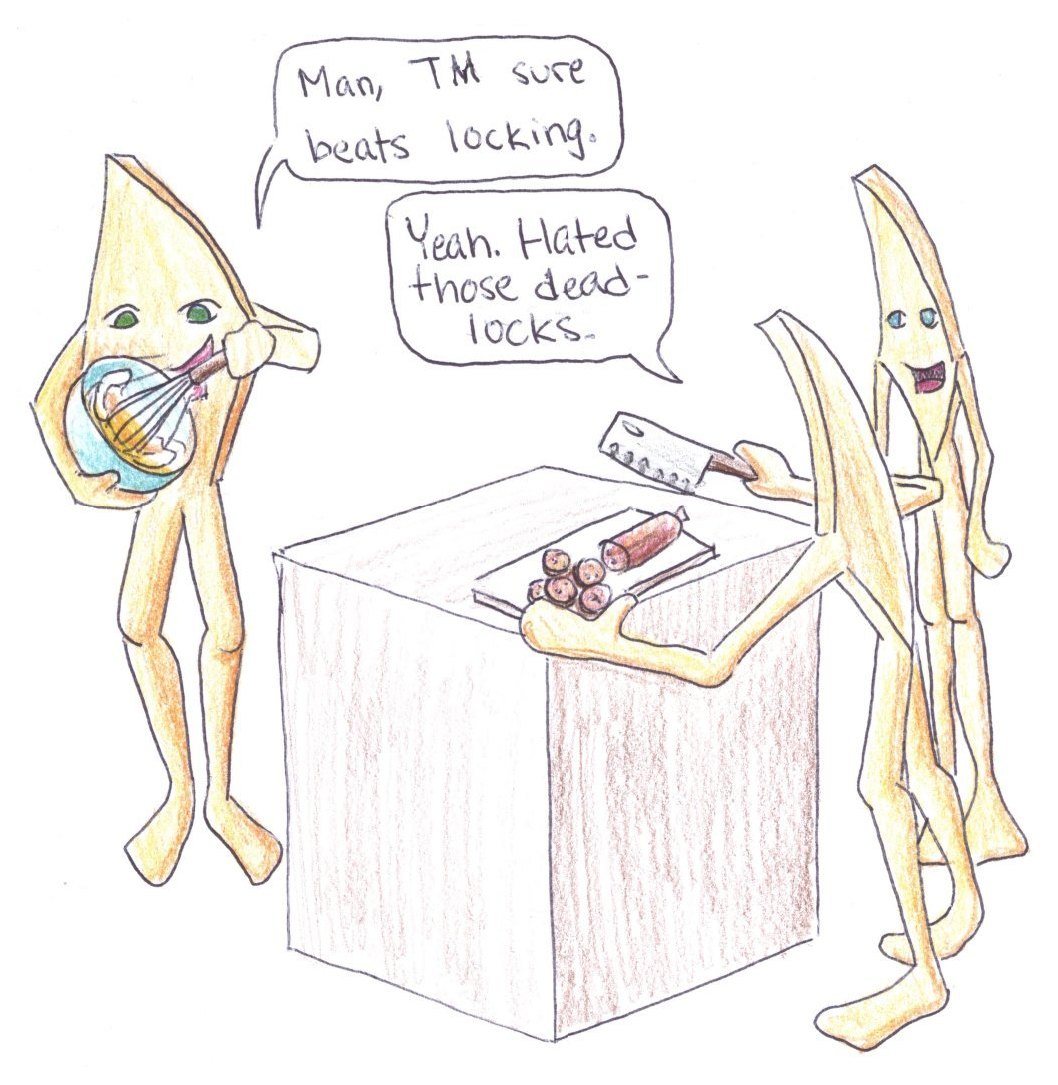
\includegraphics{cartoons/TM-the-vision}}
\caption{The STM Vision}
\ContributedBy{Figure}{fig:future:The STM Vision}{Melissa Broussard}
\end{figure}

\begin{figure}[tb]
\centering
\resizebox{3in}{!}{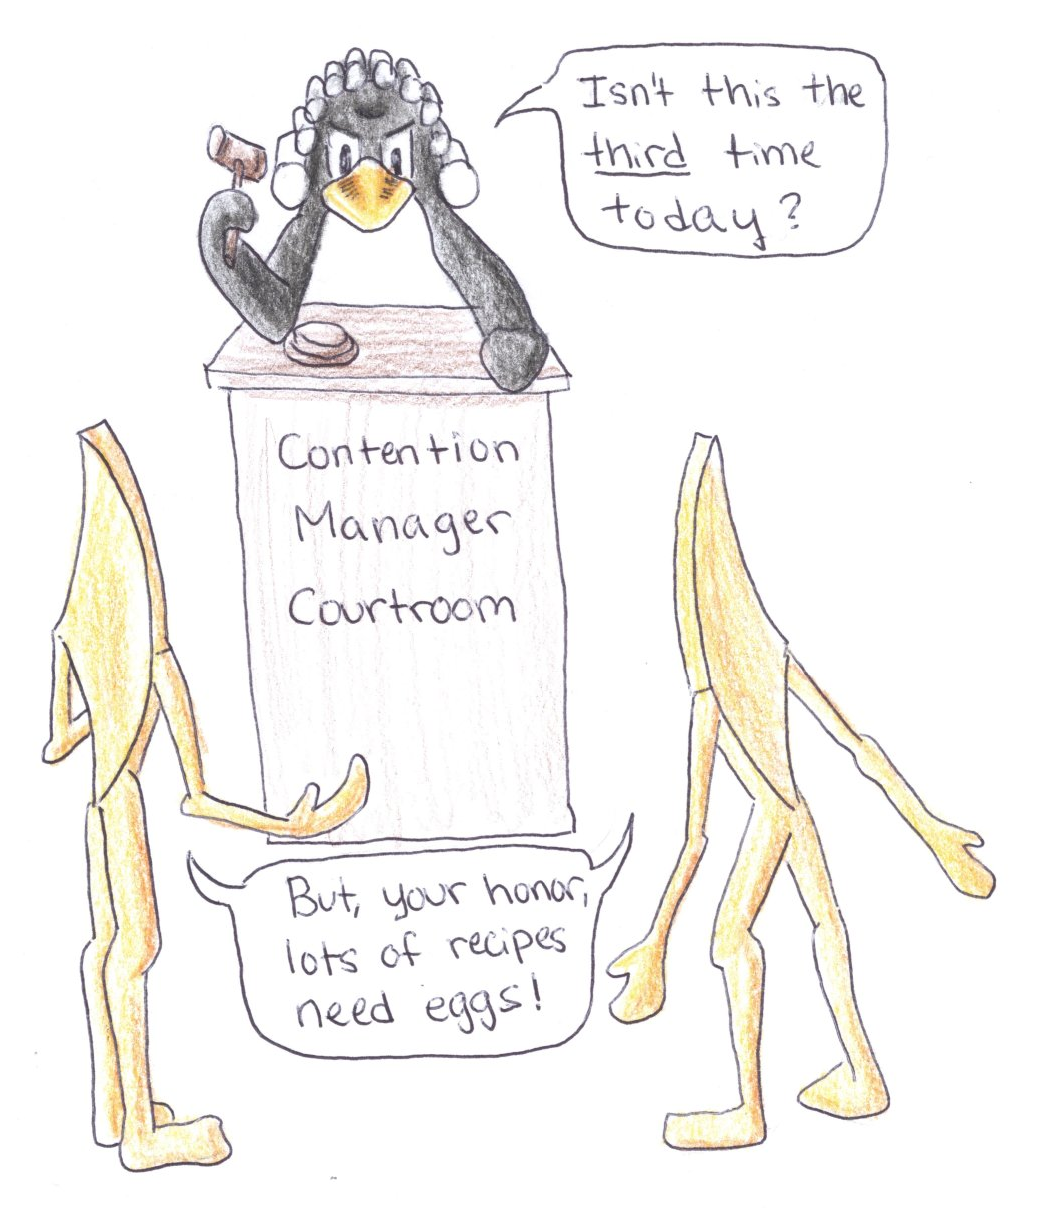
\includegraphics{cartoons/TM-the-reality-conflict}}
\caption{The STM Reality: Conflicts}
\ContributedBy{Figure}{fig:future:The STM Reality: Conflicts}{Melissa Broussard}
\end{figure}

\begin{figure}[tb]
\centering
\resizebox{3in}{!}{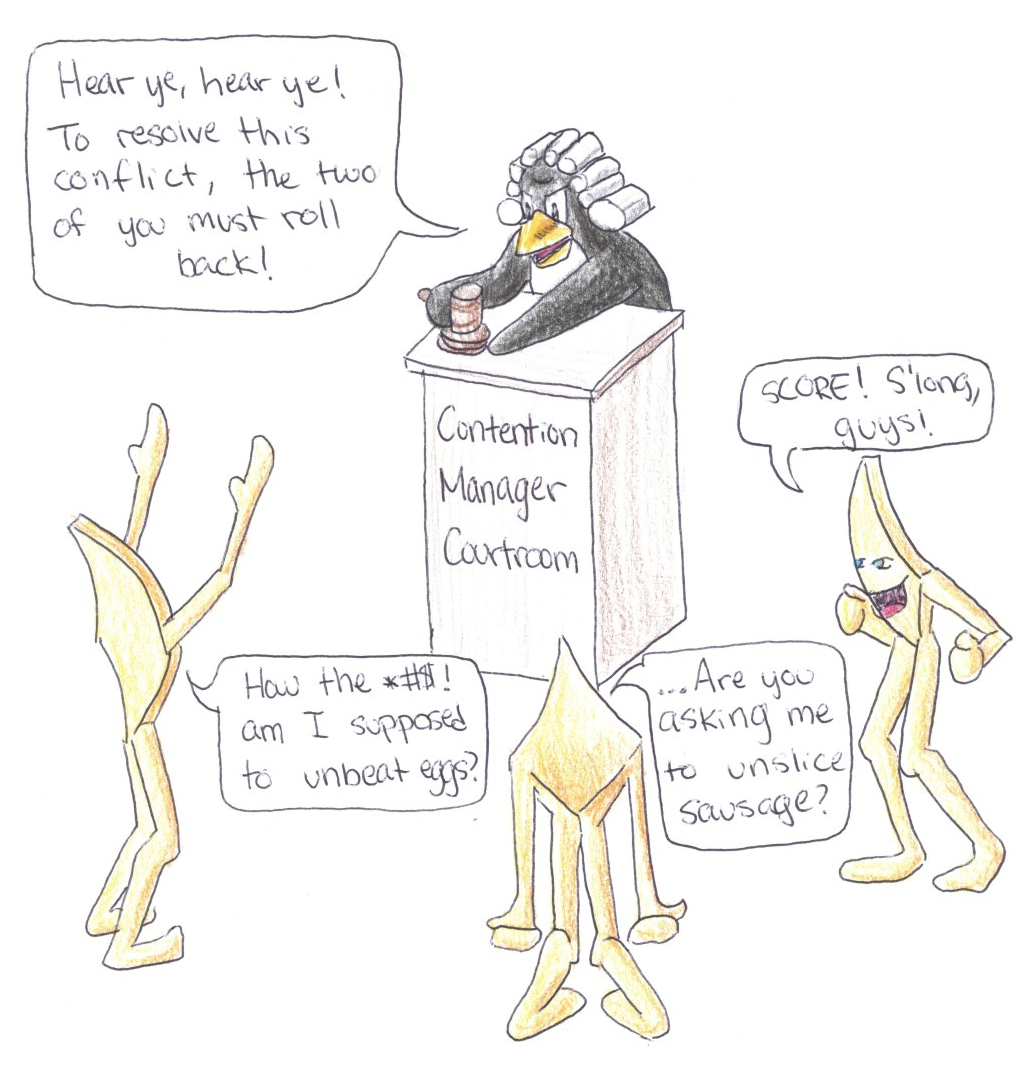
\includegraphics{cartoons/TM-the-reality-nonidempotent}}
\caption{The STM Reality: Irrevocable Operations}
\ContributedBy{Figure}{fig:future:The STM Reality: Irrevocable Operations}{Melissa Broussard}
\end{figure}

\begin{figure}[tb]
\centering
\resizebox{3in}{!}{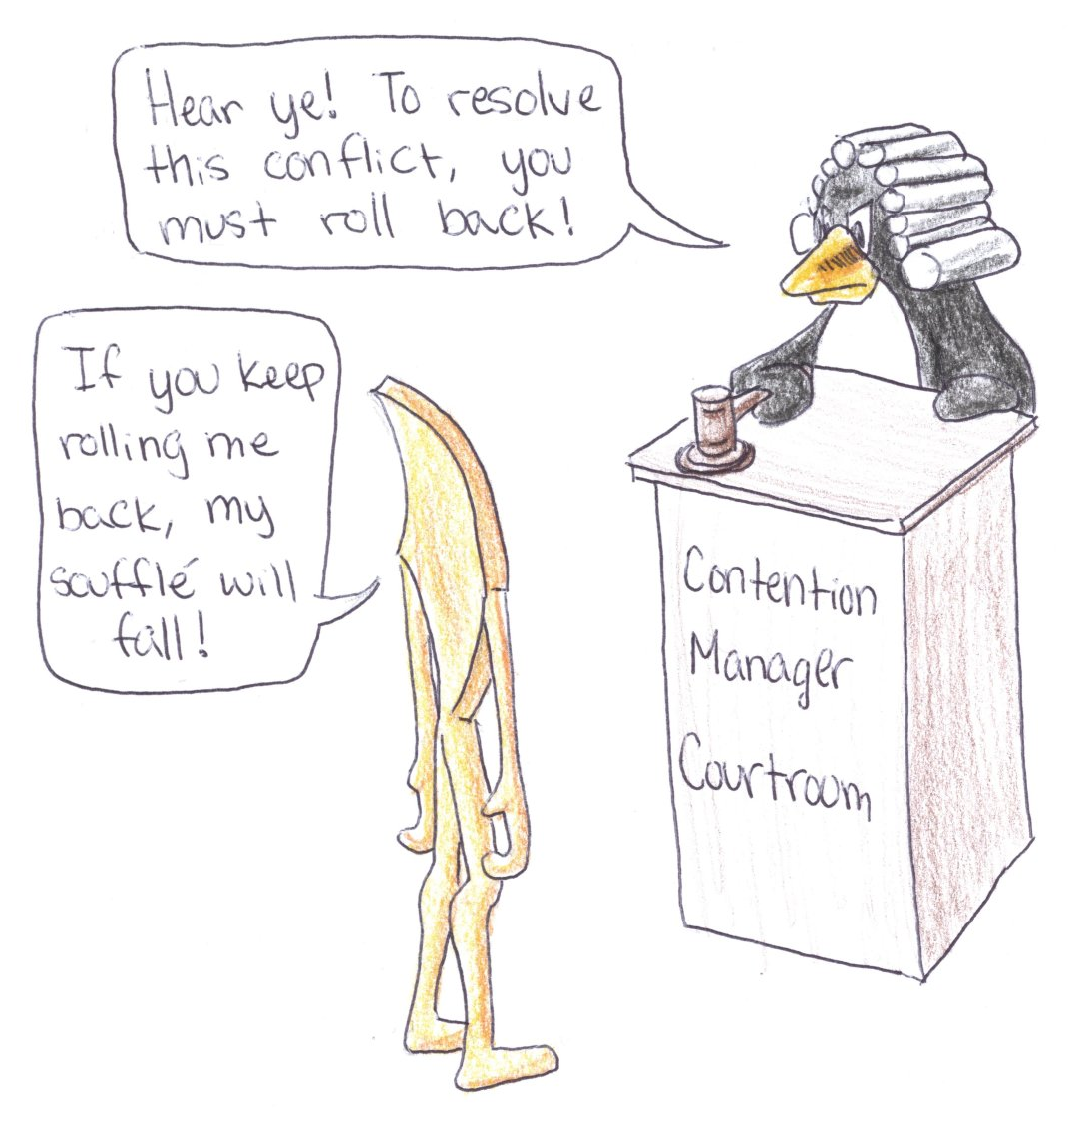
\includegraphics{cartoons/TM-the-reality-realtime}}
\caption{The STM Reality: Realtime Response}
\ContributedBy{Figure}{fig:future:The STM Reality: Realtime Response}{Melissa Broussard}
\end{figure}

But for the moment, the current state of STM
can best be summarized with a series of cartoons.
First,
Figure~\ref{fig:future:The STM Vision}
shows the STM vision.
As always, the reality is a bit more nuanced, as fancifully depicted by
Figures~\ref{fig:future:The STM Reality: Conflicts},
\ref{fig:future:The STM Reality: Irrevocable Operations},
and~\ref{fig:future:The STM Reality: Realtime Response}.

Recent advances in commercially available hardware have opened the door
for variants of HTM, which are addressed in the following section.

% @@@ Don Porter's user-level TM work for Linux.
